%% bare_conf.tex

\documentclass[10pt, conference, compsocconf]{IEEEtran}
% Add the compsocconf option for Computer Society conferences.
%
% If IEEEtran.cls has not been installed into the LaTeX system files,
% manually specify the path to it like:
% \documentclass[conference]{../sty/IEEEtran}

\usepackage{booktabs} % For formal tables
\usepackage{bm}
\usepackage{amsmath}
\usepackage{algorithm}
\usepackage{indentfirst}
\usepackage[noend]{algpseudocode}
\usepackage{multirow}
\usepackage{etoolbox}
\usepackage{siunitx}
\usepackage{graphicx}

% *** CITATION PACKAGES ***
%

\ifCLASSOPTIONcompsoc
  % IEEE Computer Society needs nocompress option
  % requires cite.sty v4.0 or later (November 2003)
  \usepackage[nocompress]{cite}
\else
  % normal IEEE
  \usepackage{cite}
\fi
\usepackage{cite}

% *** GRAPHICS RELATED PACKAGES ***
%
\ifCLASSINFOpdf
  % \usepackage[pdftex]{graphicx}
  % declare the path(s) where your graphic files are
  % \graphicspath{{../pdf/}{../jpeg/}}
  % and their extensions so you won't have to specify these with
  % every instance of \includegraphics
  % \DeclareGraphicsExtensions{.pdf,.jpeg,.png}
\else
  % or other class option (dvipsone, dvipdf, if not using dvips). graphicx
  % will default to the driver specified in the system graphics.cfg if no
  % driver is specified.
  % \usepackage[dvips]{graphicx}
  % declare the path(s) where your graphic files are
  % \graphicspath{{../eps/}}
  % and their extensions so you won't have to specify these with
  % every instance of \includegraphics
  % \DeclareGraphicsExtensions{.eps}
\fi

% *** MATH PACKAGES ***
%
%\usepackage[cmex10]{amsmath}
% A popular package from the American Mathematical Society that provides
% many useful and powerful commands for dealing with mathematics. If using
% it, be sure to load this package with the cmex10 option to ensure that
% only type 1 fonts will utilized at all point sizes. Without this option,
% it is possible that some math symbols, particularly those within
% footnotes, will be rendered in bitmap form which will result in a
% document that can not be IEEE Xplore compliant!
%
% Also, note that the amsmath package sets \interdisplaylinepenalty to 10000
% thus preventing page breaks from occurring within multiline equations. Use:
%\interdisplaylinepenalty=2500
% after loading amsmath to restore such page breaks as IEEEtran.cls normally
% does. amsmath.sty is already installed on most LaTeX systems. The latest
% version and documentation can be obtained at:
% http://www.ctan.org/tex-archive/macros/latex/required/amslatex/math/





% *** SPECIALIZED LIST PACKAGES ***
%
%\usepackage{algorithmic}
% algorithmic.sty was written by Peter Williams and Rogerio Brito.
% This package provides an algorithmic environment fo describing algorithms.
% You can use the algorithmic environment in-text or within a figure
% environment to provide for a floating algorithm. Do NOT use the algorithm
% floating environment provided by algorithm.sty (by the same authors) or
% algorithm2e.sty (by Christophe Fiorio) as IEEE does not use dedicated
% algorithm float types and packages that provide these will not provide
% correct IEEE style captions. The latest version and documentation of
% algorithmic.sty can be obtained at:
% http://www.ctan.org/tex-archive/macros/latex/contrib/algorithms/
% There is also a support site at:
% http://algorithms.berlios.de/index.html
% Also of interest may be the (relatively newer and more customizable)
% algorithmicx.sty package by Szasz Janos:
% http://www.ctan.org/tex-archive/macros/latex/contrib/algorithmicx/




% *** ALIGNMENT PACKAGES ***
%
%\usepackage{array}
% Frank Mittelbach's and David Carlisle's array.sty patches and improves
% the standard LaTeX2e array and tabular environments to provide better
% appearance and additional user controls. As the default LaTeX2e table
% generation code is lacking to the point of almost being broken with
% respect to the quality of the end results, all users are strongly
% advised to use an enhanced (at the very least that provided by array.sty)
% set of table tools. array.sty is already installed on most systems. The
% latest version and documentation can be obtained at:
% http://www.ctan.org/tex-archive/macros/latex/required/tools/


%\usepackage{mdwmath}
%\usepackage{mdwtab}
% Also highly recommended is Mark Wooding's extremely powerful MDW tools,
% especially mdwmath.sty and mdwtab.sty which are used to format equations
% and tables, respectively. The MDWtools set is already installed on most
% LaTeX systems. The lastest version and documentation is available at:
% http://www.ctan.org/tex-archive/macros/latex/contrib/mdwtools/


% IEEEtran contains the IEEEeqnarray family of commands that can be used to
% generate multiline equations as well as matrices, tables, etc., of high
% quality.


%\usepackage{eqparbox}
% Also of notable interest is Scott Pakin's eqparbox package for creating
% (automatically sized) equal width boxes - aka "natural width parboxes".
% Available at:
% http://www.ctan.org/tex-archive/macros/latex/contrib/eqparbox/





% *** SUBFIGURE PACKAGES ***
%\usepackage[tight,footnotesize]{subfigure}
% subfigure.sty was written by Steven Douglas Cochran. This package makes it
% easy to put subfigures in your figures. e.g., "Figure 1a and 1b". For IEEE
% work, it is a good idea to load it with the tight package option to reduce
% the amount of white space around the subfigures. subfigure.sty is already
% installed on most LaTeX systems. The latest version and documentation can
% be obtained at:
% http://www.ctan.org/tex-archive/obsolete/macros/latex/contrib/subfigure/
% subfigure.sty has been superceeded by subfig.sty.



%\usepackage[caption=false]{caption}
%\usepackage[font=footnotesize]{subfig}
% subfig.sty, also written by Steven Douglas Cochran, is the modern
% replacement for subfigure.sty. However, subfig.sty requires and
% automatically loads Axel Sommerfeldt's caption.sty which will override
% IEEEtran.cls handling of captions and this will result in nonIEEE style
% figure/table captions. To prevent this problem, be sure and preload
% caption.sty with its "caption=false" package option. This is will preserve
% IEEEtran.cls handing of captions. Version 1.3 (2005/06/28) and later 
% (recommended due to many improvements over 1.2) of subfig.sty supports
% the caption=false option directly:
%\usepackage[caption=false,font=footnotesize]{subfig}
%
% The latest version and documentation can be obtained at:
% http://www.ctan.org/tex-archive/macros/latex/contrib/subfig/
% The latest version and documentation of caption.sty can be obtained at:
% http://www.ctan.org/tex-archive/macros/latex/contrib/caption/




% *** FLOAT PACKAGES ***
%
%\usepackage{fixltx2e}
% fixltx2e, the successor to the earlier fix2col.sty, was written by
% Frank Mittelbach and David Carlisle. This package corrects a few problems
% in the LaTeX2e kernel, the most notable of which is that in current
% LaTeX2e releases, the ordering of single and double column floats is not
% guaranteed to be preserved. Thus, an unpatched LaTeX2e can allow a
% single column figure to be placed prior to an earlier double column
% figure. The latest version and documentation can be found at:
% http://www.ctan.org/tex-archive/macros/latex/base/



%\usepackage{stfloats}
% stfloats.sty was written by Sigitas Tolusis. This package gives LaTeX2e
% the ability to do double column floats at the bottom of the page as well
% as the top. (e.g., "\begin{figure*}[!b]" is not normally possible in
% LaTeX2e). It also provides a command:
%\fnbelowfloat
% to enable the placement of footnotes below bottom floats (the standard
% LaTeX2e kernel puts them above bottom floats). This is an invasive package
% which rewrites many portions of the LaTeX2e float routines. It may not work
% with other packages that modify the LaTeX2e float routines. The latest
% version and documentation can be obtained at:
% http://www.ctan.org/tex-archive/macros/latex/contrib/sttools/
% Documentation is contained in the stfloats.sty comments as well as in the
% presfull.pdf file. Do not use the stfloats baselinefloat ability as IEEE
% does not allow \baselineskip to stretch. Authors submitting work to the
% IEEE should note that IEEE rarely uses double column equations and
% that authors should try to avoid such use. Do not be tempted to use the
% cuted.sty or midfloat.sty packages (also by Sigitas Tolusis) as IEEE does
% not format its papers in such ways.





% *** PDF, URL AND HYPERLINK PACKAGES ***
%
%\usepackage{url}
% url.sty was written by Donald Arseneau. It provides better support for
% handling and breaking URLs. url.sty is already installed on most LaTeX
% systems. The latest version can be obtained at:
% http://www.ctan.org/tex-archive/macros/latex/contrib/misc/
% Read the url.sty source comments for usage information. Basically,
% \url{my_url_here}.





% *** Do not adjust lengths that control margins, column widths, etc. ***
% *** Do not use packages that alter fonts (such as pslatex).         ***
% There should be no need to do such things with IEEEtran.cls V1.6 and later.
% (Unless specifically asked to do so by the journal or conference you plan
% to submit to, of course. )


% correct bad hyphenation here
\hyphenation{op-tical net-works semi-conduc-tor}

\begin{document}
\title{Multistream Classification with Heterogeneous Feature Space}


% author names and affiliations
% use a multiple column layout for up to three different
% affiliations

% \author{\IEEEauthorblockN{Bo Dong, Yifan Li, Yang Gao, Ahsanul Haque and Latifur Khan}
% \IEEEauthorblockN{
% The University of Texas at Dallas \\
% Richardson, TX \\
% Email: (bxd130630, yli, yxg122530, axh129430, lkhan)@utdallas.edu}

% \and
% \IEEEauthorblockN{Mohammad M. Masud}
% \IEEEauthorblockN{
% United Arab Emirates University\\
% Al Ain, UAE \\
% Email: m.masud@uaeu.ac.ae}
% }

\author{Anonymous Authors}

\maketitle

\begin{abstract}
Recently, a new concept of multistream is introduced. Under this problem setting, 
two data streams are involved, which are referred as source and target streams. The 
source stream continuously generates data instances from a certain domain with 
labels, while the target stream continuously generates data instances from another 
domain without labels. Existing approaches assume that domains for both data streams 
are identical, which is not quite true in reality, since data streams from different 
sources may contain distinct features. Furthermore, obtaining labels for every instance 
in data streams is often expensive and time-consuming. Therefore, whether labeled 
instances from related streams can be helpful to predict the unlabeled instances in 
a certain stream becomes an important topic to explore. In this paper, domains between 
source and target streams may have distinct feature spaces and data distributions. 
Our objective is to predict class labels of data instances in the target stream by 
using the classifiers trained in the source stream.

We propose a framework of multistream classification by incorporating domain adaptation 
between source and target streams. At the same time, empirical valuation and analysis 
on both synthetic and real-world datasets are performed to validate the effectiveness 
of our proposed algorithm, comparing to state-of-the-art techniques. Experiment results 
show that our approach significantly outperforms other existing benchmarks.
\end{abstract}

\begin{IEEEkeywords}
multistream; classification; domain adaptation; concept drift;
\end{IEEEkeywords}

% \IEEEpeerreviewmaketitle

\section{Introduction}
Data stream is a very important concept in a modern connected Internet 
world, and it has attracted the attention of researchers worldwide. Given some important
applications of data streams, such as IoT, social networks, surveillance, and etc.,
mining data streams is becoming a more and more important topic to explore. 
However, data stream mining is also a challenging task due to its distinctive nature. 
For example, a data stream is theoretically infinite in length, therefore its volume
is very large. Meanwhile, it is possible that we have high velocity of data arrivals as well. Those properties has distinguished data 
stream mining significantly from traditional data mining problems \cite{haque2016SAND}.


% This paragraph talks about stream classification
Classification techniques solve problems of identifying which of a certain set of categories
that a new instance belongs. Normally it is assumed that the classification model, which is
trained by source data with true labels, is also representative to target data.
However, this assumption doesn't always hold in real world applications. Since data streams are generated
by non-stationary processes, it is possible that arbitrary changed may be introduced to data streams during generation. 
Due to this shift in concept, using model trained by old source data may introduce bias
in prediction \cite{herlihy1993methodology}.
In this case, a classification model trained by previous data is no longer representative to test
data in the future, and will perform poorly in prediction due to bias. Thus, the model needs regular updates to adapt the current concept.
When it comes to the setting of multistream, the classification problem becomes even
more challenging. This problem setting is described and motivated by a Multistream
Classification (MSC) algorithm \cite{chandra2016adaptive}. Two data streams are
involved simultaneously under this setting. One is referred as the source stream,
which contains data instances with true output values generated from a non-stationary
process. The other is referred as the target stream, which consists data generated
from another non-stationary process. Since getting true labels for target streams needs tremendous validation by human experts, here
we assume that true labels of test stream will not be available after the prediction. This is another assumption that previous research may suffer. 

% This paragraph talks about domain adaptation
We consider a domain adaptation setting within the multistream classification framework. there is a need to address machine learning tasks of building 
models in a one domain by using information available from another domain. In
this case, knowledge from the source domain can be transferred to the target domain to
help get high prediction accuracy. This transferring process is important in many 
circumstance where labels in a certain domain are limited or too expensive to obtain \cite{arnold2007comparative, hoi2014libol}, which fits the need of multistream by nature.
For example, it is difficult to collect labeled sensor
data from personal devices, while rich information from social media messages are available, such as 
activities and locations. Thus, knowledge from social media side can be transferred to
the physical world to address the ubiquitous computing tasks \cite{wei2016instilling}. 

In practice, most existing approaches usually conduct the learning problems in batch, such as previous example, Here, it 
assumes that training data are provided as a whole in advance \cite{pan2010survey}. However, such assumption 
doesn't always hold in real world applications, since under a data stream setting 
all instances may arrive in a sequential manner. Take online spam email detection for example \cite{chen2015opinion}. 
Normally, a classifier is built in by using a static training dataset, and it is trained in batch to
detect spam emails as accurately as possible. However, the very definition of spam varies from 
person to person. In this case, the transfer of knowledge to personalize the spam detector for each 
individual becomes critical. Even for a specific person, the definition of spam could change over time. During a 
time period one may consider advertisement from Zillow to be spam. When he starts to consider buying a house,
Zillow ads is not spam for him anymore. Such problem can be formulated as an multistream learning task, the 
objective of which is to build an online prediction model for the target domain by using information 
available in the source domain with distinct feature space. Compared to the previous example, this task 
is more challenging, as the concept is evolving in the data streams simultaneously in both source and target streams.

\begin{figure}[t]
\centering
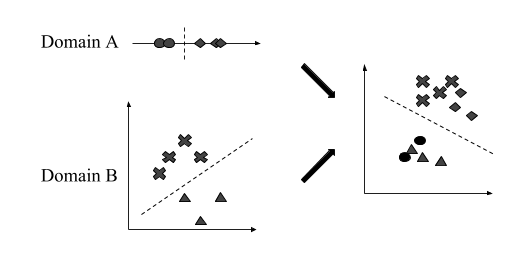
\includegraphics[width=1.0\columnwidth]{Figures/feature_projection.png}
\caption{Feature Space Projection}
\label{fig:featureprojection}
\end{figure}

This paper proposes a solution, called MultiStream Domain Adaptation (MSDA), to handle the issues described above. The
main idea is to find a common feature subspace for two distinctive streams. This idea can
be demonstrated in Figure ~\ref{fig:featureprojection}. In this case, data in domain A are 1D and in domain B are 2D. By applying the proposed projection algorithm, we
try to find a latent feature space that distribution in original and latent feature space are similar. 
Meanwhile the structure of data is preserved, which means distinct classes are still far apart.
Thus the core problem here is to find a feature space that maximize the similarity between 




\label{sec:introduction}

\section{Related Work}
There are mainly two research aspects that are related to our proposed model. 
The first one is domain adaptation, the other one is concept drift correction. The following reviews some important related work.

\subsection{Domain Adaptation}

One of fundamental assumptions in data mining, known as the ``stationary distribution assumption'', is that both the training and test data are generated from the same domain and thus represent the same data distribution~\cite{zadrozny2004learning}. Therefore, common techniques normally cannot be directly deployed when training and test data are from different domains. The differences between domains can be normally considered as two aspects: 1. distinct number of features; 2. distinct feature distributions. Several approaches have been proposed to learn a common feature representation for domain adaptation~\cite{journals/ml/Ben-DavidBCKPV10,pan2010survey}. Pan et al. ~\cite{conf/aaai/PanKY08} utilize a new dimension reduction method, Maximum Mean Discrepancy Embedding (MMDE), for domain adaptation. They try to learn a set of common transfer components underlying both domains such that the difference in distributions of data in the different domains, when projected onto this subspace, can be reduced. Shi et al.~\cite{shi2010transfer} proposed an linear objective function to project a latent feature space for both source and target domains. Both of these approaches~\cite{shi2010transfer, conf/aaai/PanKY08} focus on  static data only. Recall that in stream feature space may evolve over times across streams, which may trigger heterogeneous feature space. Zhao et al. ~\cite{zhao2010otl} uses a co-regularized method to project target domain to source domain in an online manner. However, this method also makes a strong assumption that features in source dataset is a subset of those in target dataset, which in reality, this is not always the case. However, the method works in an incremental manner which may be suitable for stream setting.

Similarly, as we stated in the last section, it is challenging to derive an online method to reduce the distribution different between domains. The state-of-the-art methods mostly address domain adaptation problems for stationary data except Zhao et al~\cite{zhao2010otl}. Thus, fitting domain adaptation frameworks to online data streams is yet to explore.



\subsection{Stream Classification}
Data stream classification is a challenging task due to its inherent properties, such as infinite length and concept drift. The infinite length problem is addressed by dividing the whole stream into fixed-size minibatches or using a gradual forgetting mechanism~\cite{journals/icdm/MasudGKHT08}. Recent approach~\cite{conf/sdm/BifetG07} address this problem by remembering only the instances within two consecutive concept drifts using a dynamically-sized minibatch. The minibatch size is increased until a concept drift is detected. Once a drift is detected, the classifier is updated and the instances representing the old concept in the minibatch are removed.

Concept drift detection in multivariate data streams concentrates on tracking any changes in the posterior class distribution, $P(y|x)$. Instead of tracking changes in $P(y|x)$ directly, the approaches proposed in~\cite{conf/sbia/GamaMCR04} adopt the principle~\cite{haque2018framework} to detect this change indirectly by tracking drift in the error rate of the underlying classifier. However, tracking drift in the error rate requires true labels of test data instances, which are scarce in practice. Recent studies focus on a feedback mechanism using prediction error~\cite{conf/sbia/GamaMCR04} or confidence~\cite{chandra2016adaptive} to detect changes in distribution between two different time windows by detecting change points in the process. Apart from working on a single stream, these methods explicitly detect change points.

The problem setting described in this paper is motivated by a Multistream Classification framework~\cite{chandra2016adaptive}. It proposes a solution which focuses on the classification problems when there are asynchronous concept drifts on source and target streams. Since stream classification is a continuous process, data in the target stream is assumed to be generated with very few labels. Yet, there are two strong assumptions made for this work: First, there is a fixed number of features in both source and target streams. Next, features have a strict one to one mapping/correspondence from source stream to target stream. However, these assumptions may not always hold in real world scenarios. To overcome those obstacles, our proposed approach does not have this latter strong assumptions. Our proposed approach assumes that domains are related (e.g., Video review vs DVD review domains), however,  features may not be exactly the same between domains, both in number and correspondence. Furthermore, other features in source stream may not have any mapping to features in target stream and vice-versa. 



\label{sec:relatedwork}

\section{Problem Formulation}
In this section, the problem of multistream classification with domain adaptation is finalized, and the challenges of conducting an adaptive classification performance over concept drifting data streams is presented.

\begin{figure}[t]
\centering
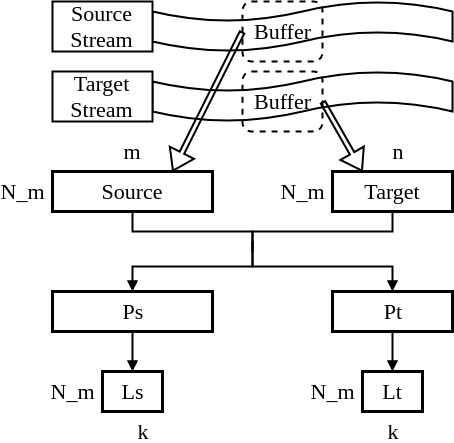
\includegraphics[width=0.7\columnwidth]{Figures/domain_adaptation.png}
\caption{Feature Projection}
\label{fig:domainadaptation}
\end{figure}


\subsection{Notations and Problem Statement}
\label{subsec: problemstatement}

In Table~\ref{tab:notations}, frequently used symbols in this paper are listed. There are two 
continuous stream of data instances generated from source domain $D_{s}$ and target domain $D_{t}$.
A data instance is denoted as $(x, y)$, where $x$ is a vector ($m$-dimensional in 
source stream and $n$-dimensional in target stream), and $y$ is the 
corresponding class label. In the source stream, both $x_{s}$ and $y_{s}$  are available, while in the target domain only $x_{t}$ is available. Therefore, a multistream classification with domain adaptation problem can be described as follows:

Suppose $X_{s}$ is a set of $m$-dimensional vectors and $Y_{s}$ is the corresponding labels in a source stream from a certain domain $D_{s}$, 
whereas $X_{t}$ is a set of $n$-dimensional vectors in target stream from another 
domain $D_{t}$. In our problem setting, $m\neq n$. The objective is to construct a classifier $M$ that
predicts class labels of $x_{t} \in X_{t}$ using $X_{s}$, and $Y_{s}$.

\begin{table}[t]
\centering
\caption{Notations}
\label{tab:notations}
\begin{tabular}{|l|l|}
\hline
Symbol & Meaning \\ \hline
 $D_{s}$ & Domain of source stream \\ \hline
 $D_{t}$ & Domain of target stream \\ \hline
 $S$ & Source stream data\\ \hline
 $T$ & Target stream data \\ \hline
 $X_{s}$, $X_{t}$ & Feature space of source stream with dimension $m$, \\
  & and that of target stream with dimension $n$\\ \hline
 $Y_{s}$, $Y_{t}$ & Label space of source and target stream \\ \hline
 $x_{s}$, $x_{t}$ & Data instance of source and target stream \\ \hline
 $y_{s}$, $y_{t}$ & True/predicted label of a data instance in source stream \\ \hline
 $W_{s}$, $W_{t}$ & Projection function to the source and target space \\ \hline
 $L_{s}$, $L_{t}$ & Projected data from source and target domain to latent space \\ \hline
 $P_{s}$, $P_{t}$ & Probability distribution function of source and target data \\ \hline 
 $N_{m}$ & Size of sliding window \\ \hline
\end{tabular}
\end{table}

\subsection{Challenges}
In the problem setting of multistream classification with domain adaptation, there are two major challenges at the same time.
The first challenge is the adaptation of both source and target domain, and it can be represented as $D_{s} \neq D_{t}$. As shown in Figure~\ref{fig:domainadaptation}, two streams may have different number of instances. However, without loss of generality, buffers (windows) from these streams representing contiguous data points will have the same number of instances $N_m$. Furthermore, each data point in source stream may have a different number of features compared to those in the target stream.

Therefore, source data cannot be directly used as training data to learn the target task, 
and discovering a latent feature space with $k$ dimensions is the key to handling the feature heterogeneity issue.
The second challenge is the asynchronous concept drift in both source and target streams. 
This phenomenon means that the data pattern evolves, or more formally, the conditional probability distribution changes over time in both streams. 
Here, the problem can be described as $P_{s}^{t}(y \mid \mathbf{x}) \neq P_{t}^{t}(y \mid \mathbf{x})$ at time $t$. Furthermore, we assume that source and target data streams have asynchronous concept drifts,
which means that the drifts in both streams occur independently. 

% \textcolor{red}{add detailed demonstration of the flow chart here}

\label{sec:problemformulation}

\section{Proposed Approach}
In this paper, we propose a Multistream Domain Adaptation (MSDA) framework to address the major issues in our problem setting. 
% \textcolor{red}{To be specific, the assumption of heterogeneous domains holds valid between source and target streams,
% while there are concept drift in both streams as well. Thus, our goal of designing this framework is to use as much information as possible from the source stream,
% to predict the instance labels in the target stream. [there's no reason to restate the problems/goals right after you stated them]}
To achieve this goal, we establish a framework with the following modules:

\begin{enumerate}
\item A domain adaptation module that helps find an optimized latent subspace for both source and target streams. 
\item A concept drift detection module that detects concept drift in both source and target streams.
\end{enumerate}

\begin{figure}[t]
\centering
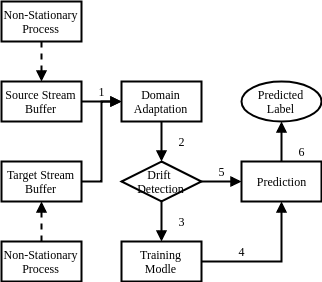
\includegraphics[width=0.7\columnwidth]{Figures/flowchart.png}
\caption{Multistream Classification with Domain Adaptation}
\label{fig:flowchart}
\end{figure}

Applying these two modules together, once a concept drift is detected, we use data instances from both streams in the most recent window to update the feature mapping, so that the domain adaptation problem can be addressed. The diagram of this algorithm can be found in Figure \ref{fig:flowchart}.

In our framework, data instances are generated simultaneously from both source and target domains. The content in parentheses correspond to contents in Figure~\ref{fig:flowchart} and Algorithm~\ref{alg::overall} respectively.

First, a domain adaptation module is triggered to learn projection functions for both source and target data instances (step 1, 2 \& line 2-6). 
Newly arriving instances are transformed to latent feature representation accordingly (line 8-11). 
Second, the change point detection module detects if there is a significant change in either source or target streams within the sliding windows  
Third, once a change point is detected, new classifiers are trained based on these two buffers from $B_s$ and $B_t$ (step 3 \& line 12-16).
Finally, the newly updated classifiers are used to  predict the labels of adapted data instances from target stream $T$ (step 4, 5, 6 \& line 17-18). Details of our proposed method is as follows.

\begin{algorithm}[t]  
\caption{MSDA Algorithm}  
\label{alg::overall}  
\begin{algorithmic}[1]  
\Require  
Labeled source stream $S$,
Unlabeled target stream $T$,  
The size of sliding window $N_m$.
Similarity parameter $\beta$.
\Ensure  
Labels predicted on $T$.
\State /* Initialization */
\State $B_s, B_t \gets readData(S,T)$
\State /* DA for initial buffer */
\State $W_s, W_t \gets genProjectionFunction(B_s, B_t, \beta)$
\State $L_s, L_t \gets genProjectionMatrix(B_s, B_t, W_s, W_t)$
\State $M \gets buildModel(L_s, Y_s)$

\While {$S$ or $T$ $exists$}
\State $B_s, B_t \gets readData(S,T)$
\State /* DA for stream buffer */
\State $W_s, W_t \gets genProjectionFunction(B_s, B_t, \beta)$
\State $L_s, L_t \gets genProjectionMatrix(B_s, B_t, W_s, W_t)$
% \State $M \gets buildModel(L_s, Y_s)$
\State /* Concept drift detection and correction */
\State Call $ChageDetection$ // Algorithm 2
\If {$ChangeDetection = True$}
\State /* Update prediction model */
\State $M \gets buildModel(L_s, Y_s)$

\EndIf
\State /* Generate predictions */
\State $\hat{y_{t}} \gets getPrediction(M,L_t)$
% \State print $getMAE (\hat{y}_t, B_t)$
\EndWhile

\end{algorithmic}  
\end{algorithm}

\subsection{Initialization and Domain Adaptation}

In our proposed framework, instances from source and target streams are stored in $B_{s}$ and $B_{t}$ respectively. 
Recalling our problem setting, data in $B_{s}$ have true labels, while data in $B_t$ come without true labels. 
The domain adaptation method is indeed a optimization problem solved by feature embedding~\cite{shi2010transfer}.
Also, for computational purposes, we design our approach in a way that buffer size in both source and target streams are the same, which means the numbers of data instances in processing window for source and target streams are identical. 
Thus, given a certain time $t$, data that we have are: source stream window matrix $B_s \in \mathds{R}^{N_m \times m}$; source stream window labels vector $Y_{s} \in \mathds{R}^{N_m \times 1}$, and; target stream window matrix $B_t \in \mathds{R}^{N_m \times n}$. 
In this case, the best projection strategy of $L_{s}$ and $L_{t}$ in the latent feature space would be the minimization of following objective function:
\begin{equation}
\label{fcn:overallMinimization}
    \mathcal{O} = \min_{L_{s}, L_{t}}\ell\left ( B_s, L_{s} \right ) + \ell\left ( B_t, L_{t} \right ) + \beta \mathbf{D}\left(L_{s}, L_{t} \right )
\end{equation}
where $\ell\left(\cdot , \cdot \right)$ is a distance function that evaluates the differences between the original data and projected data. 
$\mathbf{D}\left(\cdot, \cdot\right)$ is the co-regularizer that promotes the similarities between the two projected domains ($L_{s}$ and $L_{t}$). $\beta$ is a parameter that determines how desirable the two projected data are similar.
The first two terms are expected to preserve the structure of the original data as much as possible. 
Therefore, we define the loss function $\ell\left(\cdot, \cdot\right)$ as the Frobenius norm, which can also be expressed as a matrix trace norm $\ell\left(B_s, L_{s}\right) $ equals $\left \| B_s - L_{s}W_{s}  \right \|_{F}^2$, and $\ell\left(B_t, L_{t}\right)$ equals $ \left \| B_t - L_{t}W_{t}  \right \|_{F}^2$.

We factorize the original data into projections ($L_{s}$ and $L_{t}$) by linear mapping functions ($W_{s}$ and $W_{t}$).
Also, note that here we are not applying the alternative definition such as $\ell\left(B_s,L_{s}\right) $ as $\left \| B_{s}W_{s} - L_{s}  \right \|_{F}^2$, since this definition will always lead to a trivial solution $W_{s} = 0$ and $L_{s} = 0$, thus $B_{s}W_{s} = L_{s} = 0$ will always minimize the objective function. From Equation~\ref{fcn:overallMinimization} the projected data should preserve the structures of original data.

Furthermore, we define $\mathbf{D}\left(L{s}, L_{t}\right)$ as follows:
\begin{equation}
\label{fcn:crossSimilarity}
    \mathbf{D}\left(L_{s}, L_{t}\right) =\frac{1}{2}\left(\ell\left(B_s, L_{t}\right) + \ell\left(B_t, L_{s}\right)\right)
\end{equation}
which is the mean value of cross-similarity between the original data and projected data. Finally, the parameter $\beta$ controls the trade-off of importance of semantic similarity co-regularization by minimizing the differences between $\mathbf{D}(L_{s}, L_{t})$.

Combining Equation \ref{fcn:overallMinimization} and \ref{fcn:crossSimilarity} together, we obtain the overall optimization objective function as follows:
\begin{equation}
\label{fcn:finalObjectiveFunction}
\begin{split}
    \mathcal{O} &= \left \| B_s - L_{s}W_{s}  \right \|_{F}^2 + \left \| B_t - L_{t}W_{t}\right \|_{F}^2 \\
    &+ \frac{1}{2}\beta \left \| B_s - L_{t}W_{s}  \right \|_{F}^2 + \frac{1}{2}\beta \left \| B_t - L_{s}W_{t}\right \|_{F}^2
\end{split}
\end{equation}
% \textcolor{red}{[you maybe should expand $l(\cdot,\cdot)$ in this equation]}
Notice here the projection itself will perform rotation and scaling on the target matrix to minimize the difference.
Since $L_s$ and $L_t$ are orthogonal matrices, $B_{s}^{\top}B_{s}=1$. Also, we are applying the cyclic permutation property of trace. Thus, Equation \ref{fcn:finalObjectiveFunction} can be expanded by the representation of trace.

We therefore adopt an alternative formula to solve this problem by iteratively fixing one of the projection matrices until the remaining one converges. 
That is, we can take the derivative of $\mathcal{O}$ with regard to $W_s$ and $W_t$.
Under this conditions, our formula is defined as follows accordingly.

\begin{equation}
\begin{split}
    \frac{\partial \mathcal{O}}{\partial W_{s}} =  (2+\beta)W_{s} -2L_{s}^{\top}B_{s} - \beta L_{t}^{\top}B_{t} \\
    \frac{\partial \mathcal{O}}{\partial W_{t}} =  (2+\beta)W_{t} -2L_{t}^{\top}B_{t} - \beta L_{s}^{\top}B_{t} \\
\end{split}
\end{equation}

According to Long et al.~\cite{long2008general}, setting both partial derivatives to zero would generate the optimal solution based on KTT conditions.
Consequently, the projection function for both source and target stream can be formulated as:

\begin{equation}
\begin{split}
    W_s = \cfrac{\beta}{2+\beta} L_{t}^\top B_{s} + \cfrac{2}{2+\beta} L_{s}^\top B_{s} \\
    W_t = \cfrac{\beta}{2+\beta} L_{s}^\top B_{t} + \cfrac{2}{2+\beta} L_{t}^\top B_{t} \\
\end{split}
\end{equation}

After the steps described above, the optimal projection for both source and target stream to the latent feature space would be formed accordingly. 

% Furthermore, we need to screen the optimization to avoid mappings between two totally unrelated data. A sample selection algorithm is used to eliminate those unrelated examp/les, that is, if the source data is too different from target data, we will consider that it is ``too risky'' to conduct the domain adaptation.

%%%%%%%%%%%%%%%%%%%%%%%%%%%%%%%%%%%%%%%%%%%
% Here goes Tao's code
%%%%%%%%%%%%%%%%%%%%%%%%%%%%%%%%%%%%%%%%%%%

\subsection{Classification Module}

Initially, we train a classifier using a small set of data instances from both $S$ and $T$, which are referred to as the initialization data. The new data representation is obtained by using initialization data from $B_s$ and $B_t$ as follows:

\begin{equation}
\begin{cases}
L_s^{(i)}=B_s^{(i)}W_s^{-1} \qquad B_s^{(i)}\in B_s \\
L_t^{(j)}=B_t^{(j)}W_t^{-1} \qquad {B}_t^{(j)}\in {B}_t\\
\end{cases}
\end{equation}

There are several algorithm can be used in MSDA. As new instances arrive in $S$ or $T$, the classifier is updated if there is a drift to ensure that it represents the current concepts. A new classification model is trained using data in $B_s$ and $B_t$ at that time. Concept drift detection and the updating method used by MSDA will be discussed Section~\ref{sec:changedetection} in this section. MSDA predicts the  class label of an incoming target instance from the target stream after projecting the instance into the new data format.


\subsection{Change Detection Module (CDM)}
\label{sec:changedetection}

Previous work~\cite{chandra2016adaptive} of multistream classification uses prediction confidence to detect changes in distribution between two different time windows. Due to possible asynchronous concept drifts between source and target streams, an ensemble of classifiers is maintained and updated if a concept drift is detected in either of these streams of data. Therefore, complex ensemble algorithms may lead to very slow execution.

\begin{algorithm}[t]  
\caption{ChangeDetection: Change Detection}  
\label{alg::detection}  
\begin{algorithmic}[1]  
\Require  
Source instances $B_s=\{B_s\}^{i=1}$, target instances $B_t=\{B_t\}^{j=1}$, new instance $x$, initial mean discrepancy $Disc$, the change parameter $\tau$.
\Ensure  
$True$ if drift is detected, else $False$.
\State /* Instance is from source stream */
\If {$x \in S$}
\State $B_s^{(N_m+1)} \leftarrow x$.
\State $L_s^{(N_m+1)}=xW_s^{-1}$.
\State $B_s^{(i)} \leftarrow B_s^{(i+1)}, i=1,...,N_m$.
\State $L_{s}^{(i)} \leftarrow L_{s}^{(i+1)}, i=1,...,N_m$.
\State $\mu_S=\frac{1}{N_m} \sum_{i=1}^{N_m}  L_{s}^{(i)}W_s^{-1}$.
\State Go to line 16.
\EndIf
\State /* Instance is from target stream */
\State $B_t^{(N_m+1)} \leftarrow x$.
\State $L_{t}^{(N_m+1)}= xW_t^{-1}$.
\State $B_t^{(i)} \leftarrow B_t^{(j+1)}, j=1,...,N_m$.
\State $L_{t}^{(j)} \leftarrow L_{t}^{(j+1)}, j=1,...,N_m$.
\State $\mu_T=\frac{1}{N_m} \sum_{j=1}^{N_m} \mathbf L_{t}^{(j)} W_t^{-1}$.
\State /* Calculate the mean discrepancy $Disc_t$ at time $t$: */
\quad $Disc_t=\|\mu_s^t-\mu_t^t\|^2$.
\State $s=ln\frac{Disc_t}{Disc_0}$.
\State \bf{Return} $s>-ln(\tau)$.
\end{algorithmic}  
\end{algorithm}

We adopt the Maximum Mean Discrepancy (MMD) as the distance measure to compare different distributions. The distance between two distributions can be computed between the sample means of the two domains in the $k$-dimensional embeddings:
\begin{equation}
\begin{split}
&Disc(L_{newS},L_{newT})\\
&= \left\lVert \frac{1}{N_m}\sum_{i=1}^{N_m}  L_s^{(i)} W_{s}^{-1} - \frac{1}{N_m}\sum_{j=1}^{N_m}  L_t^{(j)} W_{t}^{-1}\right\rVert ^2
\end{split}
\end{equation}
where $L_{newS}$, $L_{newT}$ are the set of projected data points in the source and target windows.

We invoke a simple but efficient change detection method by monitoring significant changes in $B_s$ and $B_t$. Since data continuously arrives in the source and target streams, the MMD model in Equation needs to be updated also by updating the mean of adapted data points in the two windows respectively. The online updating process is given by:
\begin{equation}
\begin{cases}
L_s^{(i)}=B_s^{(i+1)}W_s^{-1} \qquad B_s^{(i)}\in B_s \\
L_t^{(j)}=B_t^{(j+1)}W_t^{-1} \qquad {B}_t^{(j)}\in {B}_t\\
\end{cases}
\end{equation}

Let $Disc_0$ be the initial value of mean discrepancy, and $Disc_t$ be the value of mean discrepancy at time $t$. $Disc_t$ is updated online as new instances arrive in $S$ or $T$. The difference between the distributions is determined by the log ration between MMD.
A drift is detected if it is more than a user-defined threshold $\tau$, as follows.
\begin{equation}
S = ln\frac{Disc_t(L_{s}^t,L{t}^t)}{Disc_0(L_{s}^0,L_{t}^0)}>\tau
\end{equation}

The efficiency of MSDA stems from the fact that in addition to estimating the projection matrix among current fixed windows, it uses the same Mean Discrepancy model for drift detection. Therefore, MSDA detects drift without adding any extra overhead.

Algorithm 2 demonstrates an online updating algorithm for change point detection. If a new instance arrived in the source stream, we update the window $L_s$ by discarding the oldest instance and storing the new instance (line 1-6). Then, new arrived data are projected into the new subspace, and the mean of source instances $\mu_s$ is updated as well in current window. Otherwise, we update the target window $L_t$ and target mean $\mu_t$ instead (line 9-13). At last, the mean discrepancy of two streams is calculate (line 15), and a change score formulated (line 16).

\subsection{Complexity Analysis}
In this approach, a new model is trained from source to target stream for every iteration of multistream classification. Thus, the time complexity of this approach depends on the classification model we used. Within the classification model, the training process, which is the updating model determines the complexity of whole algorithm.

MSDA has three modules, Domain Adaptation (DA) module, Change Point Detection (CDM) module, and classification module. The DA module learns projection matrix $W_s$ $W_t$ respectively, and from the instances stored in the source and target sliding window. Since it is a sequence of matrix transformation, the processing time is $O(kN_m)$. The time complexity of CDM module is $O(k)$. The time complexity of classification depends on the learning algorithm used as the base model. Therefore, MSDA has total time complexity of $O(kN_m+k)+f(k)$, where $f(k)$ is the time complexity for training a new classification model.



\label{sec:proposedapproach}

\section{Experiment}
\subsection{Baseline Methods}

\begin{table}
\centering
  \caption{Datasets}
  \begin{tabular}{|l|l|l|}
    % \toprule
    \hline
    Data set & \# features & \# instances\\ \hline
    USPS & 256 & 10,000\\ \hline
    MNIST & 780 & 60,000\\ \hline
    VIDEO & 100 & 5,000\\ \hline
    DVD & 200 & 30,000\\ \hline
    MUSIC & 300 & 30,000\\ \hline
    SYN01 & 100 & 10,000\\ \hline
    SYN02 & 200 & 20,000\\ \hline
    
%   \bottomrule
\end{tabular}
\label{tbl:datasets}
\end{table}

\begin{table*}[t]
\centering
\caption{Comparison of performance}
\label{tbl:performance}
\resizebox{1.4\columnwidth}{!}{%
\begin{tabular}{|l|l|l|l|l|l|}
\hline
Error Rate                & OTL    & HeMap-S & HeMap-L & MSDA-S & MSDA-L\\ \hline
USPS $\rightarrow$ MNIST  & 0.3231 & 0.3819  & 0.3904  & \textbf{0.2872} & 0.2996\\ \hline
MUSIC $\rightarrow$ DVD   & 0.3354 & 0.3606  & 0.3585  & 0.3291 & \textbf{0.3164}\\ \hline
VIDEO $\rightarrow$ MUSIC & 0.3801 & 0.4041  & 0.3972  & \textbf{0.3176} & 0.3202\\ \hline
VIDEO $\rightarrow$ DVD   & 0.3588 & 0.4028  & 0.4009  & \textbf{0.3235} & 0.3384\\ \hline
SYN01 $\rightarrow$ SYN02 & 0.3753 & 0.4183  & 0.4212  & \textbf{0.3350} & 0.3547\\ \hline
\end{tabular}
}
\end{table*}

To evaluate the effectiveness of our proposed our method MSDA, which uses embedding based methods for domain adaptation, we compare it with several state-of-the-art domain adaptation or online learning frameworks. Also, we applied two different variations of our method, which are MSDA-SVM and MSDA-LR. These two methods are different in a way that classifiers applied are SVM and Logistic Regression. The following paragraphs describe details of baseline methods.

\textbf{HeMap}. Heterogeneous Mapping (HeMap) projects data in two domains with correspondence onto a common latent space~\cite{shi2010transfer}. This method is designed as a batch training, which means both source and target data are offline. Also, this method requires class labels in the target dataset. We adapt HeMap into our problem by applying sliding windows. Meanwhile, two classifiers, SVM and LR, are also applied in this method as variations, which are referred as HeMap-S and HeMap-L respectively. 

\textbf{OTL}. Online Transfer Learning uses a co-regularized method to project target domain data into the source domain~\cite{zhao2010otl}. This method is applied in a supervised manner, which means that data in source domain are offline, while data in target domain are online. Furthermore, there is a strong assumption that features in source stream are a subset of those in target stream.

\subsection{Datasets}
\label{sec:datasets}




We use both synthetic and real-world datasets to evaluate our methods. As Table~\ref{tbl:datasets} shows, the first five datasets are publicly available, and the latter two synthetic datasets are generated by MOA~\cite{bifet2010moa}. 

\textbf{USPS}~\cite{hull1994database} and \textbf{MNIST}~\cite{lecun1998gradient} contain gray-scale images of hand-written digits collected from different sources. 
Each digit is size-normalized and centered in a fixed-size image, and each digit is a feature in these two datasets. Thus the number of features in two datasets are different due to the different resolution of the images.
In order to satisfy the concept drift assumption in this paper, we shift the concept of positive and negative classes in the middle of datasets. 
That is, in the first half of both USPS and MNIST, labels 0-4 represent ``-'' and labels 5-9 represent ``+'', while in the second half class labels 3-7 mean ``+'' and the rest class labels mean ``-''.

\textbf{MUSIC}, \textbf{DVD}, and \textbf{VIDEO} are text datasets generated by Amazon reviews based on product categories~\cite{blitzer2007biographies}. In these datasets, video has 5,000 of customer reviews, while MUSIC and DVD have 30,000 balanced customer reviews. Features are extracted directly from raw review text by implementing word2vec model trained by Google~\cite{mikolov2013efficient}. In order to use this data set in a binary classification setting, we label scores with ratings greater than 3 is defined as``+'', and those smaller than 3 are defined as ``-''. Scores that equals to 3 is discarded due to ambiguous polarity. Meanwhile, weighted average sentence embedding~\cite{arora2016simple} is applied to represent word vectors, which provide more weight to uncommon words.

\textbf{SYN01}, \textbf{SYN02} are synthetic datasets that are generated by MOA framework. These datasets are generated in a way that the number of features in SYN01 is 100 while that in SYN02 is 200, so that our domain adaptation assumption can be satisfied.

\subsection{Experiment Setup}
Our MSDA approach involves multiple parameters. We use $N_m = 400$ as our default setting in the experiment. Meanwhile, $\beta = 1$, $k = 4$, and $\tau = 0.1$ are selected to conduct our initial experiment here. The sensitivity of parameters will be discussed later in this section.

\subsection{Result Analysis}

\begin{figure*}[t]
   \centering
   \subfloat[][]{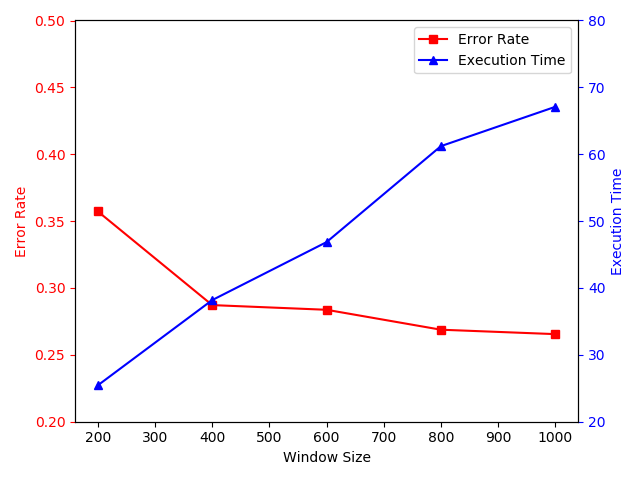
\includegraphics[width=.35\textwidth]{Figures/sen_window.png}} 
   \subfloat[][]{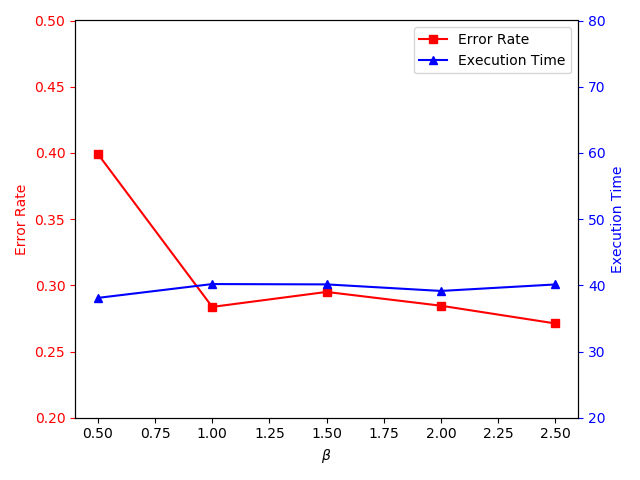
\includegraphics[width=.35\textwidth]{Figures/sen_beta.png}} \\
   \subfloat[][]{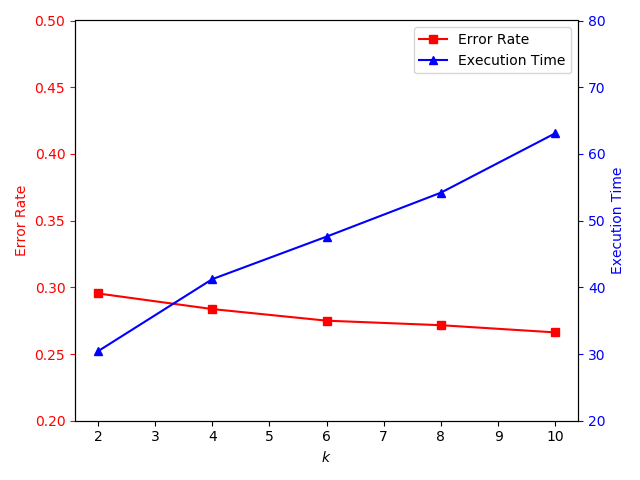
\includegraphics[width=.35\textwidth]{Figures/sen_k.png}} 
   \subfloat[][]{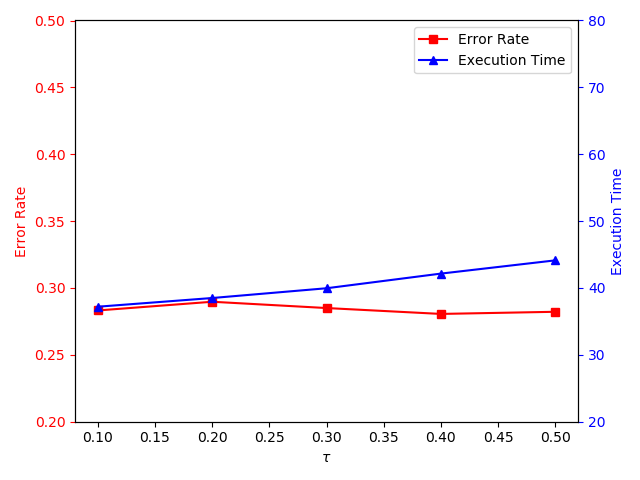
\includegraphics[width=.35\textwidth]{Figures/sen_tau.png}}
   \caption{Sensitivity Experiment Results of MSDA}
   \label{fig:sensitivity}
\end{figure*}


Table~\ref{tbl:performance} shows the average prediction error \% on the target stream $T$: $\frac{A_{wrong}}{m}$, where $A_{wrong}$ is the total number of instances identified incorrectly, and $m$ is the number of instances in the target stream. From this table, we can tell that MSDA-S outperforms all other competing methods on almost every dataset,except MUSIC $\rightarrow$ DVD. The reason here is because in other datasets information are transferred from low-dimensional to high-dimensional feature space while this dataset is reversed. Since the performance of the model can not be simply reversed, our method works better when adapting from small feature space to larger feature space. 

For example, the accuracy of OTA, HeMap-S and MSDA-S on USPS $\rightarrow$ MNIST are $32.31\%$, $38.19\%$ and $28.72\%$ respectively. 
We can see that our proposed method has better performance by a significant margin compared to baseline methods. The reason is that for OTL, the algorithm has a strong assumption that features in the source data are a subset of those in the target stream, which is not quite the case here.  
Text dataset used in this paper, such as reviews for VIDEO and DVD, would have overlapping features in terms of data distributions. However, not all features in VIDEO would exist in the DVD dataset in our settings. 
When it comes to HeMap, it also has its own shortcomings. HeMap is an offline method, which makes it not able to adapt the concept drift assumption in our problem. In this dataset specifically, the concept in the second half of data shifts from the first half of data (described in Section~\ref{sec:datasets}). Since we applied periodic updates every 4000 instances for the HeMap method, there is a delay on updating the model comparing our proposed MSDA-S approach.

\subsection{Sensitivity Analysis}
The results of our proposed method are further analyzed by tuning defined parameters $N_m$, $\beta$, $k$, and $\tau$. All experiments are conducted on USPS $\rightarrow$ MNIST dataset. In this section, we vary $N_m$ by setting it to \{200, 400, 600, 800, 1000\}, $\beta$ to \{0.5, 1, 1.5, 2, 2.5\},
$k$ to \{2, 4, 6, 8, 10\}, and  $\tau$ to \{0.1, 0.2, 0.3, 0.4, 0.5\} respectively.

First, the parameter that controls window size ($N_m$) is set to different values, and results are shown regarding how they affect MSDA approach in Figure~\ref{fig:sensitivity}. We can see that the average error decreases while the increasing window size, while the execution time increases with increasing window size. This is expected as we state that the execution time of MSDA depends on $N_m$. Based on this observation, we should choose a medium value so that both error rate and execution time could be balanced.

Second, $\beta$ determines the similarities between projected domains from both source and target stream. From Figure~\ref{fig:sensitivity}, we can tell that the error rate decreases significantly when $\beta$ increases from 0.5 to 1. If $\beta > 1$, the decreasing trend of error rate is becoming not significant. Also, we can see from the figure that the execution time regarding different $\beta$ remains similar in the experiment. Thus, we choose $\beta = 1$ as our recommended parameter here.

Third, considering the parameter that defines the dimension of latent feature space $k$. This parameter influence the model in both embedding and classification. In other words, this parameter determines how large the feature space is to apply our classifiers. From Figure~\ref{fig:sensitivity}, we can see that the performance of the model has improved marginally while the execution time increases dramatically as $k$ increases. Thus, we need to choose as small $k$ as possible, meanwhile we need to make sure that performance doesn't degrade. Thus, we choose $k = 4$ for our approach.

At last, we can see that for $\tau$, which controls the threshold for concept drift detection. In this case, the performance of model doesn't quite change when $\tau$ varies. Therefore, based on performance of execution time, we need to choose a smaller $\tau$. Hence, we select $\tau = 0.1$ in our model.

In all, those sensitivity experiments indicate that MSDA is sensitive to $N_m$ and $k$, while not quite sensitive to $\beta$ and $\tau$. 
\label{sec:experinment}

\section{Conclusions}
In this paper, a multistream classification framework that incorporates domain adaptation techniques is proposed. Two major challenges, namely heterogeneous domain and concept drift, are addressed simultaneously in two data streams.
Our solution involves an embedding-based mapping approach for domain adaptation, and an online update mechanism using average mean discrepancy for concept drift correction.
More specifically, the mapping approach helps to find a common latent space for both source and target stream, which preserves the structure of data and maximizes the similarities between source and target data.
Additionally, the prediction model is updated if a concept drift is detected, which happens when a likelihood ratio is greater than the user-defined threshold $\tau$.
Extensive experiments with both real-world and synthetic data show that our approach has significantly better performance in terms of error rate on various datasets, compared to existing state-of-the-art solutions.

We would like to extend the work in the following directions. First, we solely discuss binary classification applying SVM and LR models in this paper. We can further explore a multiple classification problems under this setting. Next, the multistream setting that we discussed in Section~\ref{sec:problemformulation} take two data streams into consideration, which are source and target data streams. A further discussion regarding three or more data streams can be explored as well. 
\label{sec:conclusions}



\bibliographystyle{IEEEref}
\bibliography{body-bibliography} 



% that's all folks
\end{document}
